\documentclass{beamer}
\usetheme{Madrid}
\usecolortheme{whale}
%\usepackage{graphicx}
%\graphicspath{{../img/}}
\usepackage[utf8]{inputenc}
\usepackage{graphicx}
\usepackage{hyperref}
\hypersetup{
	colorlinks=true,
	linkcolor=blue,
	filecolor=magenta,      
	urlcolor=cyan,
}	
\usepackage[spanish]{babel}
\usepackage{pdfpages}
\usepackage{booktabs}
\usepackage{color}

\title[Machine Learning en Cs. Sociales]{Modelos simples en Machine Learning}
\subtitle{Fundamentos de regresión logísica }
\author{German Rosati \\  \href{ german.rosati@gmail.com}{german.rosati@gmail.com}}
\institute{UNTREF - UNSAM - CONICET}
\date{\today}
%\logo{\includegraphics[height=0.4cm]{img/header-logo.png}}

\begin{document}
\frame{\titlepage}
%\begin{frame}
%	\frametitle{Hoja de ruta}
%	\tableofcontents
%\end{frame}

\section{Repaso...}
\begin{frame}
\frametitle{Repaso... }
\framesubtitle{Problemas de Clasificación}
	\begin{itemize}
		\item $Y$ es una variable cualitativa. 
		\item Toma valores sin orden en un conjunto $C$
		\item Dado un vector de features $X$ y una variable target cualitativa $Y$, un problema de clasificación busca construir una función $f(X)$ que prediga los valores de $Y$, es decir, $f(X) \in C$
		\item Muchas veces estamos interesados en un predecir \textit{probabilidades}
	\end{itemize}
\end{frame}


\section{Regresión Logística}
\subsection{Fundamentos}
\begin{frame}
	\frametitle{Regresión Logística}
	\framesubtitle{Fundamentos - Ejemplo}
		\begin{figure}[H]	
		\centering
			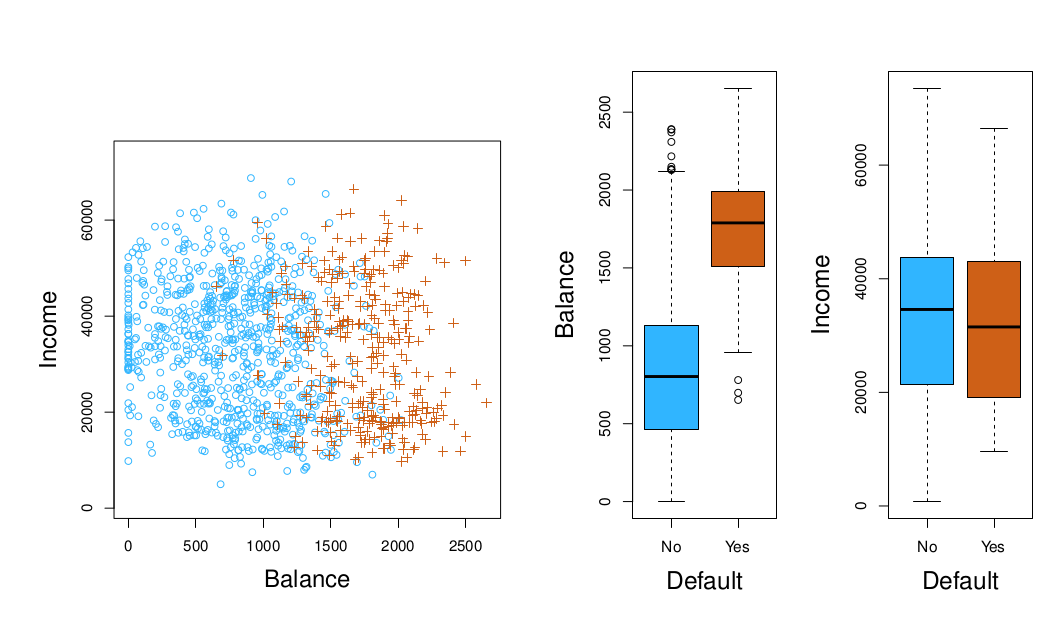
\includegraphics[width=1\linewidth, height=0.7\textheight]{./img/01}
			\caption{Scatterplot y BoxPlot Default dataset \cite{hastie02}}
		\end{figure}
\end{frame}


\begin{frame}
	\frametitle{Regresión Logística}
	\framesubtitle{¿Por qué no usar una regresión lineal?}
	\begin{itemize}
		\item Podríamos codificar $Y$ de la siguiente forma \linebreak
		
			 $
			 Y = 
				\begin{cases} 
				1 & \text{si no paga } \\
				0 & \text{si paga}
				\end{cases} 
				$
		\item ¿Podríamos realizar una regresión de $Y$ en $X$ y predecir que "SI" si $\hat{Y} \geq 0.5$?
		\item La regresión lineal produce probabilidades mayores a 1 o menores a cero. En ese sentido, una regresión logística es más apropiada.
	\end{itemize}
\end{frame}



\begin{frame}
\frametitle{Regresión Logística}
\framesubtitle{Fundamentos - Ejemplo}
\begin{figure}[H]	
	\centering
	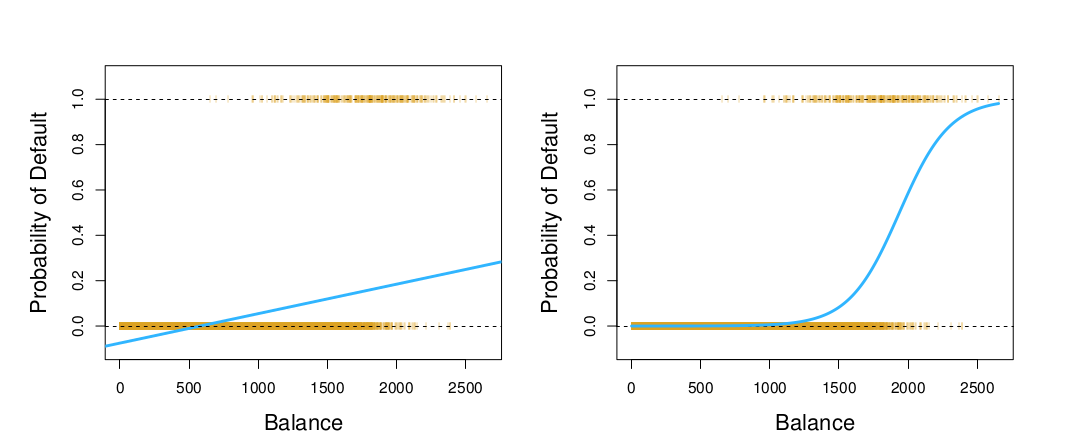
\includegraphics[width=1\linewidth, height=0.6\textheight]{./img/02}
	\caption{Regresión lineal y Logística en Default dataset \cite{hastie02}}
\end{figure}
\end{frame}

\begin{frame}
	\frametitle{Regresión Logística}
	\framesubtitle{Forma Funcional}
	\begin{itemize}
		\item Escribamos la forma de una regresión logística.
		\item Queremos predecir la probabilidad de que una persona entre en default, condicionado a los valores de otras variables $X$, y hemos codificado este evento con 1 y 0 $P(Y=1|X)$. Entonces,
		\begin{align}
			P(Y=1|X) & =  \frac{\exp^{\beta_{0} + \beta_{1}X}}{1 + \exp^{\beta_{0} + \beta_{1}X}} = \frac{1}{1+\exp^{\beta_{0} + \beta_{1}X}} \\
			P(Y=0|X) & = 1 - P(Y=1|X)
		\end{align}
		\item Independientemente del valor que tomen $\beta_{0}$ y $\beta_{1}$, $P(Y=1|X)$ nunca  va a ser mayor a 1.
		\item Por convención y para simplificar usaremos $p(X) = P(Y=1|X)$ y $1 - p(X) = P(Y=0|X)$
	\end{itemize}
\end{frame}


\begin{frame}
\frametitle{Regresión Logística}
\framesubtitle{Forma Funcional}
\begin{itemize}
	\item Tomando logaritmos y arreglando un poco la ecuación, tenemos que:
		\begin{equation}
			\log \Bigg(\frac{p(X)}{1-p(X)}\Bigg) = \beta_{0} + \beta_{1}X
	\end{equation}
	\item Esta transformación se llama log odds o logit.
\end{itemize}
\end{frame}


%\begin{frame}
%\frametitle{Regresión Logística}
%\framesubtitle{Función de Costo}
%\begin{itemize}
%	\item El "proceso que genera los datos" puede ser pensado como una distribución binomial:
%	\item Cada dato $Y_{i}$ puede tomar valores 0 o 1.
%	\item Pensemos en tirar una moneda y asignar 1 si sale cara y 0 si sale ceca.
%	\item La moneda está equilibrada, es decir, que $p(Y=1) = p(Y=0) = 0.5$.
%	\item Pero, ¿qué pasa si tiramos 3 monedas? ¿Cuál es la probabilidad de obtener 2 caras?
%	\end{itemize}
%\end{frame}
	
%\begin{frame}
%\frametitle{Regresión Logística}
%\framesubtitle{Función de Costo}
%\begin{itemize}
%	\item Son sucesos indepentientes, con lo cual, puedo plantear $P(k=2) = P(Y=1) \times P(Y=1) \times P(Y=0)$
%	\item Pero solamente calculé la probabilidad de sacar cara-cara-seca. También podría haber sacado seca-cara-cara o cara-seca-cara.
%	\item Necesito agregar una forma de calcular cuántas formas posibles hay de sacar 2 caras en 3 tiradas.
%	\end{itemize}
%\end{frame}

%\begin{frame}
%\frametitle{Regresión Logística}
%\framesubtitle{Función de Costo}
%\begin{itemize}

%	\item Generalmente, una regresión logística se estima mediante el método de Máxima Verosimilitud
%	\begin{equation}
%	P(y | p(x)) = \prod_{i=1}^n p(x)^{y_{i}} (1- p(x))^{1-y_{i}}
%	\end{equation}
%	\item Aplicando algunos logaritmos y reordenando
%	\begin{equation}
%	\log(\ell(\beta_{0}, \beta{1})) = -\sum_{i=1}^n y_{i} \log(\hat{y_{i}})  + (1-y_{i}) \log(1-\hat{y_{i})}
%	\end{equation}
%	\item Buscamos los $(\beta_{0}, \beta_{1})$, que minimicen esa función.
%\end{itemize}
%\end{frame}




\begin{frame}
\frametitle{Regresión Logística}
\framesubtitle{Función de Costo}
\begin{itemize}
	\item La idea es entrenar un vector de parámetros $( \beta_{0}, \beta_{1})$ tal que el modelo estime $p(X)$ altas para valores positivos y bajas para valores negativos. 
	\item Para un solo dato, la función de costo es 
		 \begin{equation}
		 	\ell(\beta_{0}, \beta_{1}) = 
		 		\begin{cases} 
		 			-\log(\hat{p}(x)) & \text{si } Y = 1 \\
		 			\log(1-\hat{p}(x))  & \text{si } Y = 0
		 		\end{cases} 
		 \end{equation}
	
	\item Intuición: $-\log(t)$ crece mucho cuando $t$ se acerca a 0.
	\item Costo grande si el modelo estima una probabilidad cercana a 0 para una instancia positiva, y también será muy grande si el modelo estima una probabilidad cercana a 1 para una instancia negativa
	\end{itemize}
\end{frame}


\begin{frame}
\frametitle{Regresión Logística}
\framesubtitle{Función de Costo}
\begin{itemize}
	\item $-\log(t)$ está cerca de 0 cuando $t$ está cerca de 1, entonces, el costo será cercano a 0 si la probabilidad estimada es cercana a 0 para un negativo instancia o cerca de 1 para una instancia positiva.
	\item La función de costo en todo el conjunto de entrenamiento es simplemente el costo promedio de todo el entrenamiento.
	\begin{equation}
		\ell(\beta_{0}, \beta{1}) = -\frac{1}{n}\sum_{i=1}^n \Big[y_{i} \log(\hat{p}(x))  + (1-y_{i}) \log(1-\hat{p}(x))\Big]
	\end{equation}
	\item Buscamos los $(\beta_{0}, \beta_{1})$, que minimicen esa función.
\end{itemize}
\end{frame}

\begin{frame}
\frametitle{Regresión Logística}
\framesubtitle{Predicciones}
\begin{itemize}
	\item Fiteemos una regresión lineal con la variable $balance$ -cuantitativa-
	\begin{figure}[H]	
		\centering
		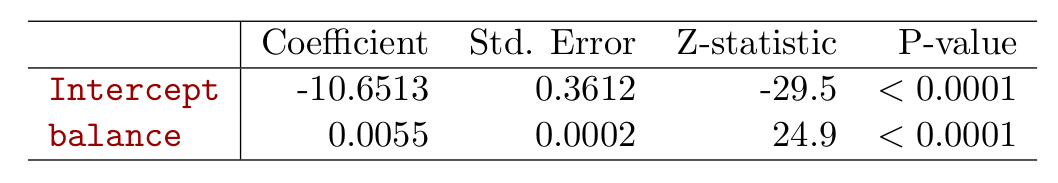
\includegraphics[width=0.9\linewidth, height=0.2\textheight]{./img/03}
		\caption{Regresión Logística en Default dataset \cite{hastie02}}
	\end{figure}
	\item ¿Qué se puede decir de estos coeficientes?
\end{itemize}
\end{frame}

\begin{frame}
\frametitle{Regresión Logística}
\framesubtitle{Predicciones}
\begin{itemize}
	\item ¿Cuál sería nuestra estimación de la probabilidad de $default$ para un $balance$ de \$1000?
	\begin{equation}
		\hat{p}(x) = \frac{exp^{\hat{\beta_{0}} + \hat{\beta_{1}}X}}{1 + exp^{\hat{\beta_{0}} + \hat{\beta_{1}X}}} = \frac{exp^{-10.6513+0.0055\times1000}}{1+exp^{-10.6513+0.0055\times1000}} = 0.006
	\end{equation}
	
		\item ¿Ypara un $balance$ de \$2000?
		\begin{equation}
			\hat{p}(x) = \frac{exp^{\hat{\beta_{0}} + \hat{\beta_{1}}X}}{1 + exp^{\hat{\beta_{0}} + \hat{\beta_{1}X}}} = \frac{exp^{-10.6513+0.0055\times2000}}{1+exp^{-10.6513+0.0055\times2000}} = 0.586
	\end{equation}
\end{itemize}
\end{frame}

\begin{frame}
\frametitle{Regresión Logística}
\framesubtitle{Predicciones}
\begin{itemize}
	\item Fiteemos una regresión lineal con la variable $student$ -cualitativa-
	\begin{figure}[H]	
		\centering
		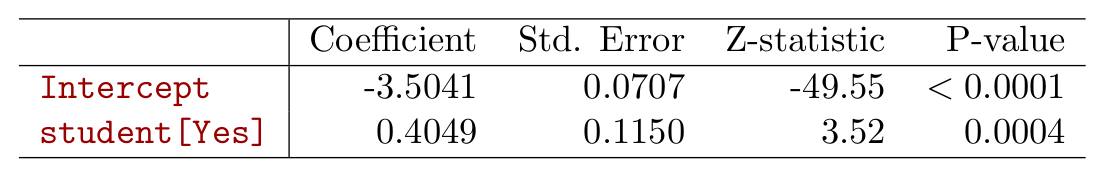
\includegraphics[width=0.9\linewidth, height=0.2\textheight]{./img/04}
		\caption{Regresión Logística en Default dataset \cite{hastie02}}
	\end{figure}
	\item ¿Qué se puede decir de estos coeficientes?
\end{itemize}
\end{frame}

\begin{frame}
\frametitle{Regresión Logística}
\framesubtitle{Predicciones}
\begin{itemize}
	\item ¿Cuál sería nuestra estimación de la probabilidad de $default$ para los estudiantes $student=1$?
	\begin{equation}
	\hat{p}(default=1 | student=1) =  \frac{exp^{-3.5041+0.4049\times1}}{1+exp^{-3.5041+0.4049\times1}} = 0.0431
	\end{equation}
	
	\item ¿Y para los no estudiantes $student=0$?
	\begin{equation}
	\hat{p}(default=1 | student=1)= \frac{exp^{-3.5041+0.4049\times0}}{1+exp^{3.5041+0.4049\times0}} = 0.0292
	\end{equation}
\end{itemize}
\end{frame}



\begin{frame}
\frametitle{Regresión Logística}
\framesubtitle{Múltiples variables}
	\begin{align}
		\log \Bigg(\frac{P(Y=1|X)}{1-P(Y=1|X)}\Bigg) = & \beta_{0} + \beta_{1}X_{1} + \beta_{2}X_{2} + ... + \beta_{p}X_{p} \\
		P(Y=1 | X) = & \frac{exp^{\beta_{0} + \beta_{1}X_{1} + \beta_{2}X_{2} + ... + \beta_{p}X_{p}}}{1+exp^{\beta_{0} + \beta_{1}X_{1} + \beta_{2}X_{2} + ... + \beta_{p}X_{p}}}
	\end{align}
	\begin{figure}[H]	
		\centering
		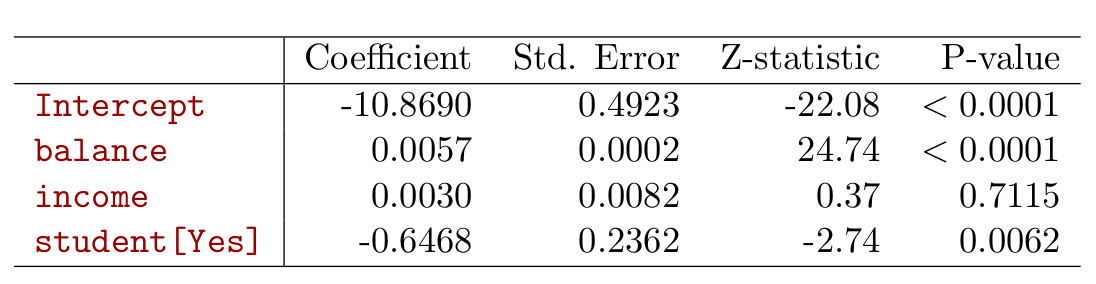
\includegraphics[width=0.9\linewidth, height=0.25\textheight]{./img/05}
		\caption{Regresión Logística en Default dataset \cite{hastie02}}
	\end{figure}
\end{frame}

\begin{frame}
\frametitle{Regresión Logística}
\framesubtitle{Múltiples variables}
\begin{itemize}
	\item Los estudiantes tienden a tener balances mayores que los no estudiantes. Por lo cual, las tasas de default "crudas" son mayores.
	\item Pero una vez que controlamos por el balance... entonces, los estudiantes defaultean menos.
\end{itemize}
\end{frame}

\begin{frame}
\frametitle{Regresión Logística}
\framesubtitle{Múltiples categorías en $Y$}
\begin{itemize}
	\item Cuando $Y$ presenta más de dos valores se fitea una regresión para cada una de las $k$ clases. 
	
	\begin{equation}
	P(Y=k | X) = \frac{\exp^{\beta_{0k} + \beta_{1k}X_{1} + \beta_{2k}X_{2} + ... + \beta_{pk}X_{p}}}{\sum_{k=1}^K \exp^{\beta_{0k} + \beta_{1k}X_{1} + \beta_{2k}X_{2} + ... + \beta_{pk}X_{p}}}   
	\end{equation}
	
	\item Es decir, se fitean $K-1$ regresiones logísticas binarias.
\end{itemize}
\end{frame}

\begin{frame}
\frametitle{Regresión Logística}
\framesubtitle{Ejercicio}
Con el dataset data\_filt.csv
\begin{enumerate}
	\item Generar una variable $Y$ que divida en 
	
	$ Y = \begin{cases} 
			1 & \text{si } p47t \geq 6990 \\
			0 & \text{si } p47t < 6990 
		\end{cases} 
	$
	\item Generar features cualitativas de forma correcta
	\item Entrenar una regresión logística para predecir 
	\item Evaluarla... (de forma correcta...)
\end{enumerate}
\end{frame}



\subsection{Overfitting}
\begin{frame}
	\frametitle{Modelo Lineal y Overfitting}
	\framesubtitle{Regularización}
	\begin{itemize}
		\item{¿Qué hacemos con el overfitting?}
		\item{Una forma es hacer \emph{model selection}...}
		\item{Otra es utilizar técnicas de regularización.}
		\item{El objetivo es introducir una restricción en la función de costo ($RSS$ - la función que se minimiza) y con eso forzar a los $\beta$} a reducir su valor \\
		\item{\textbf{Ridge:} 
			\begin{equation}
			CF = \sum_{i=1}^N(y_{i}-\beta_{0}\sum_{j=1}^p\beta_{j}x_{ij})^2 + \lambda\beta_{j}^2 = RSS + \lambda\beta_{j}^2
			\end{equation}}	
		\item{\textbf{LASSO:} 
			\begin{equation}
			CF = \sum_{i=1}^N(y_{i}-\beta_{0}\sum_{j=1}^p\beta_{j}x_{ij})^2 + \lambda|\beta_{j}| = RSS + \lambda|\beta_{j}|
			\end{equation}}	
	\end{itemize}
\end{frame}





\begin{frame}
	\frametitle{Modelo Lineal y Overfitting}
	\framesubtitle{Regularización}
	\begin{itemize}
		\item{Se parte de la minimización de $RSS$ habitual + una restricción $\lambda|\sum_{j=1}^p\beta_{j}|$ que tiene el efecto de reducir los coeficientes $\beta_{j}$ estimados}
		\item{$\lambda$ es un hiperparámetro del modelo que controla el impacto de la penalización y se estima mediante \emph{cross validation}}
		\item{Ridge se inventó originalmente para lidiar con el problema de la multicolinealidad. Sesga los coeficientes para reducir la varianza}
		\item{Ambos ``encogen'' los coeficientes hacia cero. LASSO, además, hace que algunos sean iguales a cero}
		\item{LASSO, entonces, realiza \emph{model selection}}
		\item{Es una formalización de un proceso que muchas veces se hace artesanalmente}
	\end{itemize}
\end{frame}


\begin{frame}[allowframebreaks] %allow to expand references to multiple frames (slides)

	\frametitle{Referencias bibliográficas}
		\scriptsize{\bibliographystyle{acm}}
		\bibliography{../bib/biblio} %bibtex file name without .bib extensio	n
\end{frame}



\end{document}